% !TeX program = pdfLaTeX
\documentclass[12pt]{article}
\usepackage{amsmath}
\usepackage{graphicx,psfrag,epsf}
\usepackage{enumerate}
\usepackage{natbib}
\usepackage{listings}
\usepackage{textcomp}
\usepackage[hyphens]{url} % not crucial - just used below for the URL
\usepackage{hyperref}

\providecommand{\tightlist}{%
  \setlength{\itemsep}{0pt}\setlength{\parskip}{0pt}}

%\pdfminorversion=4
% NOTE: To produce blinded version, replace "0" with "1" below.
\newcommand{\blind}{0}

% DON'T change margins - should be 1 inch all around.
\addtolength{\oddsidemargin}{-.5in}%
\addtolength{\evensidemargin}{-.5in}%
\addtolength{\textwidth}{1in}%
\addtolength{\textheight}{1.3in}%
\addtolength{\topmargin}{-.8in}%

\begin{document}

\def\spacingset#1{\renewcommand{\baselinestretch}%
{#1}\small\normalsize} \spacingset{1}


%%%%%%%%%%%%%%%%%%%%%%%%%%%%%%%%%%%%%%%%%%%%%%%%%%%%%%%%%%%%%%%%%%%%%%%%%%%%%%

\if0\blind
{
  \title{\bf Excuse me, do you have a moment to talk about version control?}

  \author{
        Jennifer Bryan \thanks{The author gratefully acknowledges the constructive feedback from
reviewers Nicholas Horton, Colin Rundel, and Hadley Wickham.} \\
    RStudio and the Department of Statistics, University of British Columbia\\
      }
  \maketitle
} \fi

\if1\blind
{
  \bigskip
  \bigskip
  \bigskip
  \begin{center}
    {\LARGE\bf Excuse me, do you have a moment to talk about version control?}
  \end{center}
  \medskip
} \fi

\bigskip
\begin{abstract}
Abstract abstract abstract.
\end{abstract}

\noindent%
{\it Keywords:} version control
\vfill

\newpage
\spacingset{1.45} % DON'T change the spacing!

\subsection{Why Git?}\label{why-git}

Why would a statistician use a version control system, such as
\href{http://git-scm.com}{Git} \citep{git}? And what is the point of
hosting your work online, e.g., on \href{https://github.com}{GitHub}
\citep{github}? Could the gains possibly justify the inevitable pain?

I say yes, with the zeal of the converted.

There are many benefits of using hosted version control in your
statistical practice:

\begin{itemize}
\tightlist
\item
  Doing your work becomes tightly integrated with organizing, recording,
  and disseminating it. It's not a separate, burdensome task you are
  tempted to neglect.
\item
  Collaboration is much more structured, with powerful tools for
  asynchronous work and managing versions.
\item
  The marginal effort required to create a web presence for a project is
  negligible.
\item
  GitHub makes a fantastic course management system for courses that use
  R \citep{R}. You can exchange actual working code with your students
  and explore the associated results.
\item
  By using common mechanics across work modes (research, teaching,
  analysis), you achieve basic competence quickly and avoid the
  demoralizing forget-relearn cycle.
\end{itemize}

Now the bad news: Git was built neither for the exact usage described
here, nor for broad usability. You will undoubtedly notice this, so it's
best to know in advance. Happily, there are many helpful tools that
mediate your interactions with Git. GitHub itself is a fine example, as
is \href{https://www.rstudio.com/products/rstudio/}{RStudio}. In
addition to pointing out tools that soften Git's sharpest edges, I
recommend specific habits and attitudes that reduce frustration.

\subsection{What is Git?}\label{what-is-git}

\href{http://git-scm.com}{Git} is a \textbf{version control system}. Its
original purpose was to help groups of developers work collaboratively
on big software projects. Git manages the evolution of a set of files --
called a \textbf{repository} or \textbf{repo} -- in a sane, highly
structured way. It is like the ``Track Changes'' feature from Microsoft
Word, but more rigorous, powerful, and scaled up to multiple files.

Git has been re-purposed by the data science community
\citep{Ram2013, git-for-humans, ten-simple-rules-git}. We use it to
manage the motley collection of files that make up typical data
analytical projects, which consist of data, figures, reports, and, yes,
source code. Even those who identify more as statistician than data
scientist generally have a similar mix of files that are the artifacts
of a project.

A lone ranger, working on a single computer, can benefit from adopting
version control. But not nearly enough to justify the pain of
installation and workflow upheaval. There are much easier ways to get
versioned back ups of files, if that's all you're worried about.

In my opinion, \textbf{for new users}, the pros of Git only outweigh the
cons when you consider the overhead of working with other people,
including your future self. And who among us does not need to do that?
In a Git-based workflow, you document and, optionally, expose your work
as you go. Communication and collaboration are the killer apps of
version control. Git's model of file management can feel uncomfortably
rigid, but it enables the distribution of files across different people,
computers, and time.

This has an implication for selecting your first Git projects: you will
enjoy the most gain for your pain if you pick a project that involves
sharing rapidly evolving files with others. It is tempting to pick a
quiet, private project, but you risk missing out on the main benefits of
formal version control.

Many people who don't use Git unwittingly re-invent a poor man's version
of it. Figure \ref{fig:diy-vs-git} depicts a hypothetical analysis of
the iris data, captured in a single R source file. With informal version
control, contributors create derivative copies of \texttt{iris.R},
decorating the file name with initials, dates, and other descriptors.
Even when working alone, this leads to multiple versions of
\texttt{iris.R} of indeterminate relatedness (Figure
\ref{fig:diy-vs-git}A). In collaborative settings based on email
distribution, the original file swiftly becomes the root of a
complicated phylogeny that no amount of ``Track changes'' and good
intentions can resolve Figure \ref{fig:diy-vs-git}B).

\begin{figure}
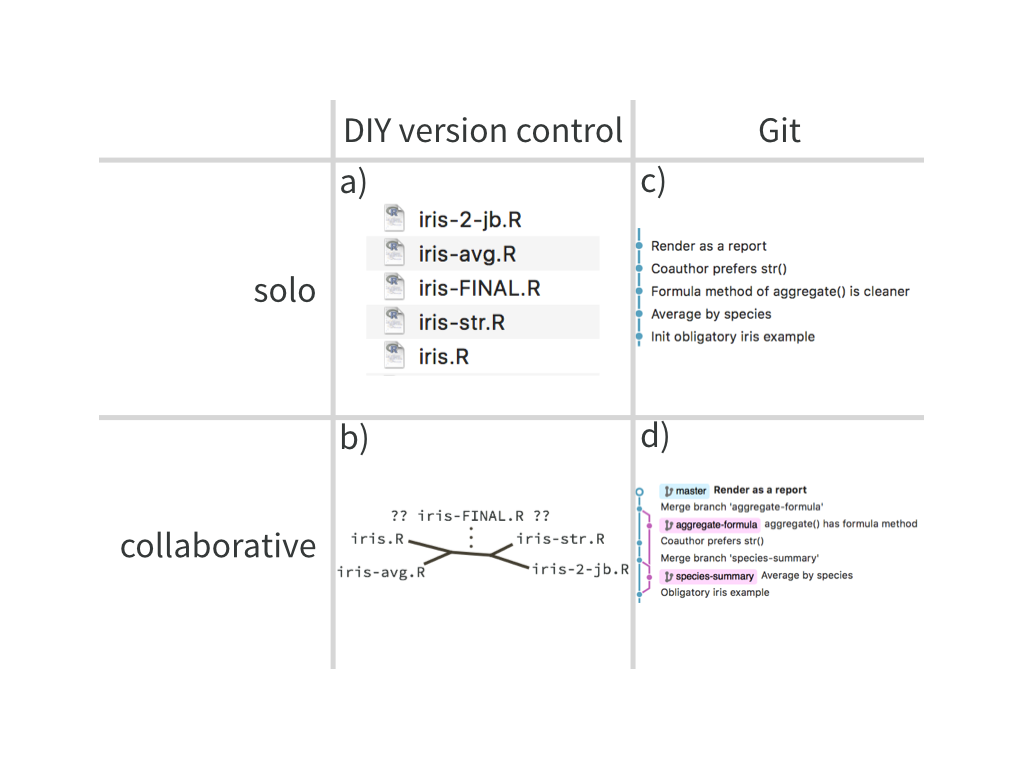
\includegraphics[width=1\linewidth]{diy-vs-git-solo-vs-collab} \caption{\label{fig:diy-vs-git}A: Solo work with DIY version control via filename. B: Collaborative work with DIY version control. C: Solo work with Git. D: Collaborative work with Git.}\label{fig:diy-vs-git}
\end{figure}

The Git way is to track the evolution of \texttt{iris.R}, through a
series of commits, each equipped with an explanatory message. Figure
\ref{fig:diy-vs-git}C depicts this linear, \emph{in situ} development
process. Figure \ref{fig:diy-vs-git}D shows the same history for a
common collaborative Git workflow, where contributors work independently
but sync regularly to a common version. Especially important versions
get a human-readable tag, to signal a meaningful milestone. Yes, there
is some pain in adopting the formalism of Git, but it is worth it.

\subsection{Who should read this and what to
expect}\label{who-should-read-this-and-what-to-expect}

The target reader is anyone who does statistical research, analysis, or
instruction. Those whose work is some combination of these three may
find the work style described here especially rewarding.

This article does not provide step-by-step instructions on how to use
Git and GitHub. This format would not be effective, but annotated links
to such resources are given in the supplementary materials. Instead, I
convey what the workflow feels like and what the payoffs are, with
special attention to the statistics and R context. The goal is to help
the Git-curious generate the activation energy needed to get started.

\subsection{What is GitHub?}\label{what-is-github}

We've explored Git's powerful structure for file management, so where
does GitHub fit in? \href{https://github.com}{GitHub} complements Git by
providing a slick user interface and distribution mechanism for Git
repositories. Git is the software you will use locally to record changes
to a set of files. GitHub is a hosting service that provides a Git-aware
home for such projects on the internet. These relationships are shown in
Figure \ref{fig:yours-theirs-github}. GitHub is like DropBox or Google
Drive, but more structured, powerful, and programmatic.

The remote host acts as the distributor for a Git-managed project. This
allows others to browse project files, explore their history, sync up
with the current version, and perhaps even propose or make changes.
GitHub's well-designed web interface is a dramatic improvement over
traditional Unix Git servers. Many operations can be done entirely in
the browser, including editing or adding files. It is easy to create a
hyperlink to a specific file or location in a file, at a specific
version, which can make meta-conversations about project code or reports
much more productive. GitHub also offers granular control over who can
see, edit, and administer a project.

\begin{figure}
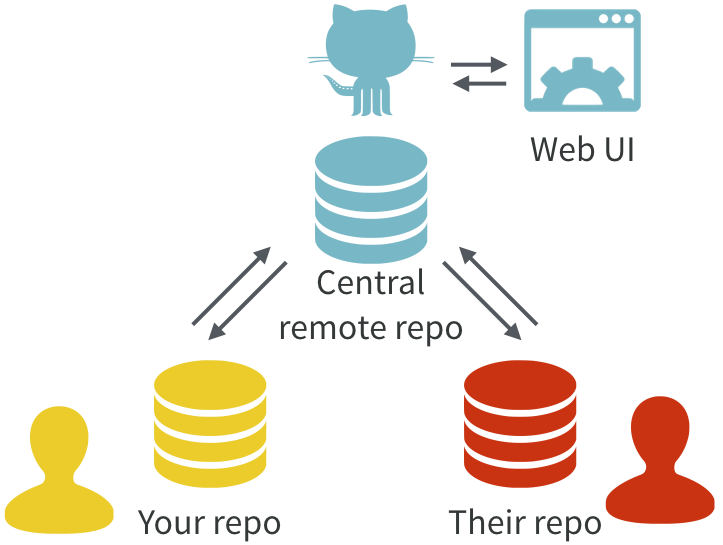
\includegraphics[width=1\linewidth]{your-repo-their-repo-central-remote-repo} \caption{\label{fig:yours-theirs-github}With Git, all contributors have a copy of the repo, with all files and the full history. It is typical to stay in sync through the use of a central remote repo, such as GitHub. Hosted remotes like GitHub also provide access to the repo through a web browser.}\label{fig:yours-theirs-github}
\end{figure}

Even for private solo projects, there are two advantages to keeping a
synced copy on GitHub:

\begin{enumerate}
\def\labelenumi{\arabic{enumi}.}
\item
  When you are new with Git (or, frankly, even when you're not), it's
  common to goof up the Git infrastructure for a project. Note that your
  files can be intact and safe, even while the Git tracking is a bit
  confused. Of course there are official Git remedies, but sometimes the
  easiest fix is to clone a fresh copy from GitHub, patch things up with
  the changes that only exist locally, and move on with your life. This
  workaround obviously requires the existence of a recent copy on
  GitHub.
\item
  The highly functional web interfaces mentioned above are often the
  most pleasant and natural way to navigate and search your files, even
  though all the same information exists locally. It is a pleasure to
  browse through your own work, across multiple projects or files and
  across time, as if it's a well-designed website. You must push your
  work to GitHub to enjoy this.
\end{enumerate}

\textbf{GitHub issues} are another powerful feature of the platform.
Recall that we are repurposing Git, a tool that facilitates software
development. Think of the issues for a project as its bug tracker. For
projects that are not pure software development, we co-opt this
machinery to organize our to-do list more generally. The basic unit is
an issue and you can interact with one in two ways.

First, issues are integrated into the project's web interface on GitHub,
with a rich set of options for linking to project files and incremental
changes. Second, issues and their associated comment threads appear in
your email, just like regular messages (this can, of course, be
configured). The result is that all correspondence about a project comes
through your normal channels, but is also tracked inside the project
itself, with excellent navigability and search capabilities. For
software, issues are used to track bugs and feature requests. In a data
analysis project, you might open an issue to flesh out a specific
sub-analysis or to develop a complicated figure. In a course, we use
them to manage homework submission, marking, and peer review.

Issues can be assigned to specific people and they can be labelled, e.g.
``bug'', ``simulation-study'', or ``final-exam''. Coupled with the
ability to cross-link issues and the project files or file changes, you
have extraordinary power to document why things have happened in the
past and to organize what needs to happen in the future.

\subsection{Initial system setup}\label{initial-system-setup}

If I've convinced you to experiment with Git and GitHub, you need to do
some initial setup. These first steps happen once or, for some steps,
once per computer. This is excerpted from
\href{http://happygitwithr.com}{Happy Git and GitHub for the useR},
which holds battle-tested instructions honed over several years in
\href{http://stat545.com}{STAT 545} at the University of British
Columbia.

\begin{itemize}
\item
  Register for a free account with GitHub.
\item
  Install Git. Depending on your OS, Git might already be installed. But
  many will need to install it or will choose to update to a more recent
  version. Some basic configuration is critical, such as setting your
  username and email.
\item
  Install a local Git client, \emph{optional but highly recommended}. A
  Git client provides a graphical user interface for Git, which is
  otherwise command-line only. If you are an R user, you will find that
  \href{https://www.rstudio.com/products/rstudio-desktop/}{RStudio}
  provides a great deal of this functionality. There are some notable
  gaps, however, so you might still choose to install a dedicated and
  comprehensive Git client such as
  \href{https://www.sourcetreeapp.com}{SourceTree} or
  \href{https://www.gitkraken.com}{GitKraken}. Git just operates on
  files, so you can do some operations from RStudio, others from
  SourceTree, and others from the shell.
\item
  Confirm, with a practice repository, that local Git can send and
  receive the current version of the repository on GitHub, known as
  \textbf{pushing} and \textbf{pulling}, respectively.
\end{itemize}

Once this setup is done, you are ready to start using Git and GitHub
with your projects. Some general recommendations for agony reduction:

\begin{itemize}
\tightlist
\item
  I repeat: consider using a graphical front-end for Git, a.k.a. a Git
  client, versus restricting yourself to the command line interface.
\item
  Establish confidence in the basics (e.g.~make a change, commit it,
  push it) before wading into more advanced usage (e.g.~branching).
\item
  Commit yourself to Git usage on a project that will provide sustained
  practice over several months. Usage in a course is great, because it
  provides a relentless stream of small deadlines.
\item
  Realize that no one is giving out Git style points. It's ok to
  ``power-cycle'', i.e.~re-initialize the Git repository, to get
  unstuck.
\end{itemize}

\subsection{Repositories and workflow}\label{repositories-and-workflow}

For new or existing projects, you will:

\begin{itemize}
\tightlist
\item
  Dedicate a local directory or folder to it.
\item
  Make it an RStudio Project. \emph{Optional but recommended; obviously
  only applies to projects involving R and users of RStudio.}
\item
  Make it a Git repository.
\end{itemize}

This setup happens once per project and can happen at project inception
or at any later point. Chances are your project already lives in a
dedicated directory. Making this directory an RStudio Project and Git
repository boils down to allowing those applications to leave notes for
themselves in hidden files or directories. The project is still a
regular directory on your computer, that you can locate, name, move, and
generally interact with as you wish. You don't have to handle it with
special gloves!

Here is the daily workflow:

\begin{itemize}
\tightlist
\item
  Go about your usual business, writing R scripts or authoring reports
  in LaTeX or R Markdown. But instead of only \emph{saving} individual
  files, periodically you make a \textbf{commit}, which takes a snapshot
  of all the files in the entire project.

  \begin{itemize}
  \tightlist
  \item
    If you have ever versioned a file
    \href{http://www.phdcomics.com/comics/archive.php?comicid=1531}{by
    adding your initials or the date}, you have effectively made a
    commit, albeit only for a single file. It is a version that is
    significant to you and that you might want to inspect or revert to
    later.
  \end{itemize}
\item
  Push commits to GitHub periodically.

  \begin{itemize}
  \tightlist
  \item
    This is like sharing a document with colleagues on DropBox or
    sending it out as an email attachment. By pushing to GitHub, you
    make your work and all your accumulated progress accessible to
    others.
  \end{itemize}
\end{itemize}

This is a moderate change to your normal, daily workflow. It feels weird
at first, but quickly becomes second nature. In
\href{http://stat545.com}{STAT 545} students are required to submit all
coursework via GitHub, starting in week one. Most have never seen Git
before and do not identify as programmers. It is a major topic in class
and office hours for the first two weeks. Then we practically never
discuss it again.

\subsection{Commits, diffs, and tags}\label{commits-diffs-and-tags}

We now connect the fundamental concepts of Git to the data science
workflow:

\begin{itemize}
\tightlist
\item
  repository
\item
  commit
\item
  diff
\end{itemize}

Recall that a repository or repo is just a directory of files that Git
manages holistically. A commit functions like a snapshot of all the
files in the repo, at a specific moment. Under the hood, that is not
exactly how Git implements things. Although mental models don't have to
be accurate in order to be useful, in this case it helps to align the
two.

\begin{figure}
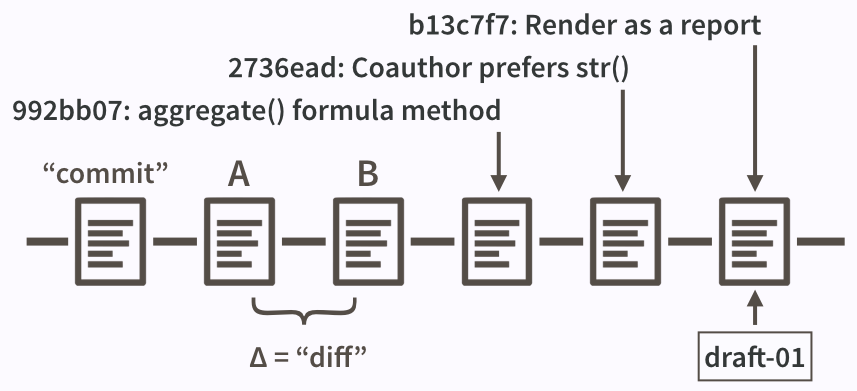
\includegraphics[width=1\linewidth]{commit-diff-sha-tag} \caption{\label{fig:commit-diff-sha-tag}Partial commit history for our iris example, highlighting diffs, commit messages, SHAs, and tags.}\label{fig:commit-diff-sha-tag}
\end{figure}

Figure \ref{fig:commit-diff-sha-tag} is another look at our fictional
analysis of the iris data, focusing on the evolution of its script,
\texttt{iris.R}. Consider version A of this file and a modified version,
version B. Assume that version A was part of one Git commit and version
B was part of the next commit. The set of differences between A and B is
called a ``diff'' and Git users contemplate diffs a lot. Diff inspection
is how you re-explain to yourself how version A differs from version B.
Diff inspection is not limited to adjacent commits. You can inspect the
diffs between any two commits.

In fact, Git's notion of any specific version of \texttt{iris.R} is as
an accumulation of diffs. If you go back far enough, you find the commit
where the file was created in the first place. Every later version is
stored by Git as that initial version, plus all the intervening diffs in
the history that affect the file. We'll set these internal details aside
now, but understanding the importance of these deltas will make Git's
operations less baffling in the long run.

So, by looking at diffs, it's easy to see how two snapshots differ, but
what about the why?

Every time you make a commit you must also write a short \textbf{commit
message}. Ideally, this conveys the motivation for the change. Remember,
the diff will show the content. When you revisit a project after a break
or need to digest recent changes made by a colleague, looking at the
\textbf{history}, by reading commit messages and skimming through diffs,
is an extremely efficient way to get up to speed. Figure
\ref{fig:commit-diff-sha-tag} shows the messages associated with the
last three commits.

Every commit needs some sort of nickname, so you can identify it. Git
does this automatically, assigning each commit what is called a SHA, a
seemingly random string of 40 letters and numbers (it is not, in fact,
random but is a SHA-1 checksum hash of the commit). Though you will be
exposed to these, you don't have to handle them directly very often and,
when you do, usually the first 7 characters suffice. The commit messages
in Figure \ref{fig:commit-diff-sha-tag} are prefixed by such truncated
SHAs. You can also designate certain snapshots as special with a
\textbf{tag}, which is a name of your choosing. In a software project,
it is typical to tag a release with its version, e.g., ``v1.0.3''. For a
manuscript or analytical project, you might tag the version submitted to
a journal or transmitted to external collaborators. Figure
\ref{fig:commit-diff-sha-tag} shows a tag, ``draft-01'', associated with
the last commit.

\subsection{Markdown is special on
GitHub}\label{markdown-is-special-on-github}

This may seem unrelated to Git, GitHub, and R, but it is now necessary
to talk about
\href{https://daringfireball.net/projects/markdown/syntax}{Markdown}.
Markdown is a markup language, like HTML and LaTeX, but designed to be
as lightweight as possible. The goal is still to separate form and
content, but also to prioritize human-readability, even at the cost of
fancy features. Markdown is in wide use on sites like
\href{https://en.support.wordpress.com/markdown/}{WordPress},
\href{https://stackoverflow.com/editing-help}{StackOverflow}, and, yes,
\href{https://help.github.com/categories/writing-on-github/}{GitHub}.
These sites use Markdown because it allows a diverse population of site
users to author decent-looking web content, with hyperlinks and some
formatting. Do not build this up into some heroic, LaTeX-level learning
task, for it is not. If you can write an email, you can write Markdown.

Any file written in Markdown is rendered in an HTML-like way on GitHub.
In particular, formatting and links ``just work''. This is the last
piece we need to seal my claim that merely pushing your project to
GitHub gives it a web presence for zero extra work. If you make even a
modest effort to embed a few explanatory Markdown files in your repo,
you will get an automatically-updated project website for free. In
particular, if a directory has a \texttt{README.md} file, GitHub renders
it like a home page or ``index.html'' when people visit that directory
in the browser. It is very common for a repo to have a top-level
\texttt{README.md}, but each subdirectory can have its own as well.

\subsection{Markdown is special for R
users}\label{markdown-is-special-for-r-users}

Markdown is especially holy for R users because of
\href{http://rmarkdown.rstudio.com}{R Markdown}, which is just Markdown
that includes chunks of R code. Figure \ref{fig:report-from-r-or-rmd}A
shows a simple \texttt{.Rmd} document for our iris example. Again, do
not regard R Markdown as something you must clear your schedule to
learn. If you can write email and a bit of R code, you can write R
Markdown. The
\href{https://CRAN.R-project.org/package=rmarkdown}{rmarkdown package}
\citep{rmd-pkg} converts R Markdown (\texttt{.Rmd} files) to Markdown
(\texttt{.md} files), running the code and inserting the results,
including figures, into the document. This is powered by another
package, \href{https://CRAN.R-project.org/package=knitr}{knitr}
\citep{knitr-pkg, knitr-book}, under the hood. This process is made
especially easy in RStudio, but is by no means limited to users of that
application. Any R user can call \texttt{rmarkdown::render("foo.Rmd")}.

\begin{figure}
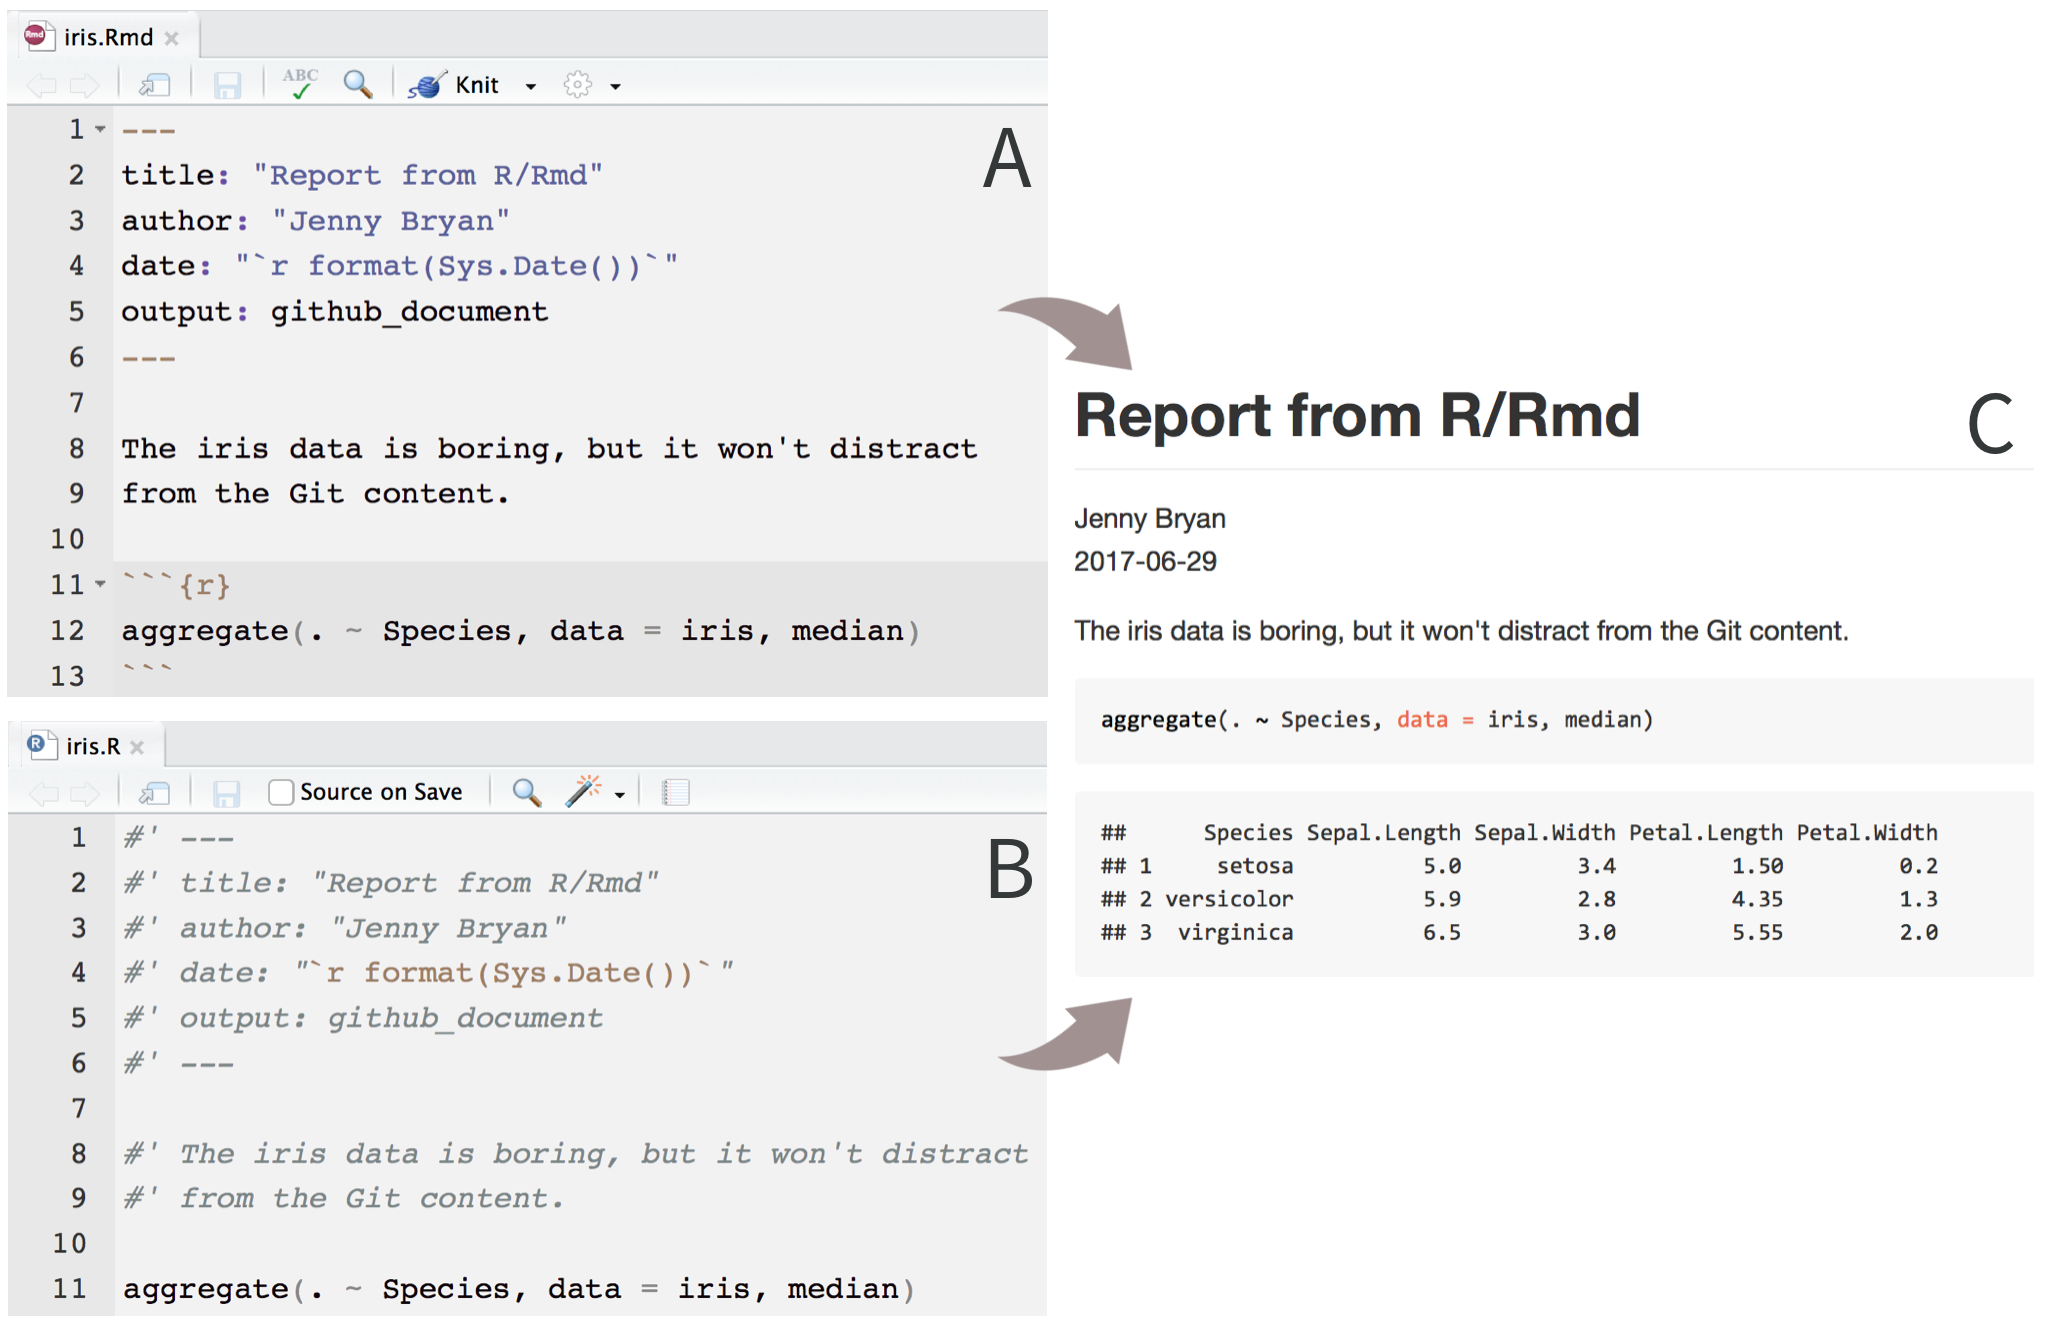
\includegraphics[width=1\linewidth]{report-from-r-or-rmd} \caption{\label{fig:report-from-r-or-rmd}A: R Markdown. B: R script, equivalent to the R Markdown in A. C: The same rendered result is produced by A or B. This is how the Markdown will look on GitHub.}\label{fig:report-from-r-or-rmd}
\end{figure}

These R-derived Markdown files, if committed and pushed, then enjoy the
usual privileged treatment on GitHub already described above. Once an
\texttt{.Rmd} file has been rendered to \texttt{.md}, anyone viewing it
on GitHub can read the prose, study the R code, \textbf{and view the
results of running that code}, including figures. Figure
\ref{fig:report-from-r-or-rmd}C shows how the \texttt{.Rmd} document
from Figure \ref{fig:report-from-r-or-rmd}A looks when rendered to
\texttt{.md} and pushed to GitHub. It is the best of all worlds, because
the code is revealed and, by definition, is the code that produced the
results. And yet a reader can gaze upon the product in a web browser,
without needing to download the code, install all necessary
dependencies, and run it.

The overall effect is that a directory that is a GitHub-synced Git repo
can simultaneously be the code-heavy back end of a project and an
outward-facing front end.

You do not, in fact, even need to work in R Markdown to exploit this. It
\href{http://rmarkdown.rstudio.com/articles_report_from_r_script.html}{works
with plain R scripts} as well. You can use exactly the same machinery to
prepare a rendered version of an R script, i.e.~to go from \texttt{.R}
to \texttt{.md}. Figure \ref{fig:report-from-r-or-rmd}B shows an R
script that produces exactly the same rendered report, i.e.~Figure
\ref{fig:report-from-r-or-rmd}C, as the R markdown in Figure
\ref{fig:report-from-r-or-rmd}B. Again, RStudio makes this especially
easy, but is not required. Once the Markdown file is pushed to GitHub,
it is as if the reader has run your code or is able to look over your
shoulder at your R session. This provides a lightweight system for
exposing work-in-progress to collaborators, without slowing down to
create separate reports. Comment lines that begin with
\texttt{\#\textquotesingle{}} are elevated to top-level prose, providing
a way to make the document more welcoming for a reader. Once there are
many prose comments, you might decide to switch from \texttt{.R} to
\texttt{.Rmd}, have proper top-level prose, and move the code down into
chunks.

Before we move on, I want to zoom out and revisit R Markdown and the
rmarkdown package more generally. Note that R Markdown can be rendered
to many more formats than Markdown, including HTML, PDF, and Microsoft
Word, and can incorporate code chunks in many languages other than R.
Markdown is emphasized here because it is extraordinarily useful in
GitHub-hosted projects. Many people are used to targetting other output
formats and overlook this special synergy between Markdown and GitHub.

\subsection{Which files to commit}\label{which-files-to-commit}

The files in a project arise in different ways and play different roles.
A critical issue for workflow happiness is to decide how to handle
different file types with respect to Git. You can direct Git to ignore
specific files or file types, such as autosaves created by your editor.
This reduces noise and clutter: Git will not pester you to commit
changes to these files and they will not appear in your GitHub
repository. A file that Git does not ignore is said to be
\textbf{tracked}. Here's a useful framework for deciding what to track:

\textbf{Source files:} These files are created and edited by hand, such
as R scripts and R Markdown or LaTeX files. This could also include the
raw data for an analysis.

\textbf{Configuration files:} These files modify the behavior of a tool,
for example \texttt{.gitignore} identifies files Git should not track
and \texttt{some-project.Rproj} records RStudio project settings.

\textbf{Derived products:} These files are programmatically generated
from source files and have external value. By executing \texttt{.R} or
rendering \texttt{.Rmd} files, you obtain artifacts such as intermediate
data (e.g., \texttt{.csv} or \texttt{.rds}), figures (e.g.,
\texttt{.png} or \texttt{.pdf}), and reports (e.g., \texttt{.md},
\texttt{.pdf}, \texttt{.docx}, or \texttt{.html}).

\textbf{Intermediates:} These files are programmatically generated and
serve a temporary purpose, but are not intrinsically valuable (e.g.,
\texttt{.aux} and \texttt{.log} in LaTex workflows).

There is clear consensus that source files should be tracked. It is also
common to track project-specific configuration files and to ignore
intermediates. However, reasonable people can disagree about how to
handle derived products and whether a specific file is an intermediate
or derived product. Therefore, the main takeaway is to pick a policy
that works for you and adapt as your needs change. There is no right
answer. I would err on the side of committing more rather than less at
first. What else should you consider when choosing files to track with
Git and share on GitHub?

\textbf{Is it useful to someone?} If so, track and share! There is a
taboo against committing derived products, inherited from Git's software
development roots, because the typical product in that context is a
platform-specific executable. This rationale, however, does not apply to
many data science products. Rendered reports, figures, and cleaned data
are often extremely valuable to others. Make them readily available.

\textbf{Will it play nicely with Git/GitHub?} This boils down to whether
Git diffs will be informative and whether GitHub has nice handling for
the file type. Small-to-medium plain text files with hard line breaks
are ideal, but there are a few more pleasant surprises.

\begin{itemize}
\tightlist
\item
  Some derived files are too miserable to read casually, such as
  \texttt{.csv} files of processed results or \texttt{.html} derived
  from \texttt{.Rmd}, yet they are still worth tracking with Git. When
  you re-run an analysis with updated input data or after updating R
  packages, \emph{the diffs are often quite modest} and help you
  pinpoint unexpected changes.
\item
  GitHub has excellent
  \href{https://help.github.com/categories/working-with-non-code-files/}{support
  for a variety of non-code files}, such as CSV and TSV. It also
  \href{https://help.github.com/articles/rendering-and-diffing-images/}{displays
  and provides visual diffs} for the most common image formats, which is
  extremely useful for spotting unexpected changes in figures.
\end{itemize}

\textbf{Will it actively cause problems with Git/GitHub?} This boils
down to the file's likely effect on Git operations. A file that is large
and changing often can make your repository bloated and slow down pushes
and pulls. If a file is binary, such as a Word document or Excel
spreadsheet, you will not get human-readable diffs anyway, nor can
GitHub display the content in the browser. Binary files are also a
reliable source of merge conflicts (see below), because they are beyond
the reach of Git's sophisticated automatic merging logic. A large binary
file that changes often is, therefore, the worst of all worlds. This
implies that adoption of Git/GitHub suggests a pivot away from
\texttt{.docx}, \texttt{.xlsx}, and \texttt{.pdf} as primary file
formats and towards \texttt{.Rmd}, \texttt{.md}, and \texttt{.csv}, at
least during periods of rapid development.

\subsection{Collaboration}\label{collaboration}

Collaboration is the most compelling reason to manage a project with Git
and GitHub. My definition of collaboration includes hands-on
participation by multiple people, including your past and future self,
as well as an asymmetric model, in which some people are active makers
and others only read or review.

Consider two different ways to collaborate on a document:

\begin{itemize}
\item
  \textbf{Edit, save, attach.} In this workflow, everyone has one (or
  more!) copies of the document, which circulate as email attachments,
  accumulating initials and dates in the filename. Which one is
  ``master''? Does this question even make sense anymore?!? If you want
  a version combining the edits made by different authors to different
  sections, how do you reconcile the copies into one? All of this
  usually gets sorted out by social contract, a fairly manual process,
  and at least one miserable person.
\item
  \textbf{Google Doc.} In this workflow, there is only one copy of the
  document and it lives in the cloud. Anyone can access the most recent
  version on demand. Anyone can edit or comment or propose a change and
  this is immediately available to everyone else. Anyone can see who's
  been editing the document and how and, if disaster strikes, can revert
  to a previous version. A great deal of ambiguity and annoying
  reconciliation work has been designed away.
\end{itemize}

Managing a project via Git/GitHub is much more like the Google Doc
scenario, but also offers some of the attractive features of ``edit,
save, attach''. With Git/GitHub, collaborators can work offline and
there can be independent lines of development, i.e.~branches. The killer
feature is that Git/GitHub enables regular and structured reconciliation
of all versions of all the files in the project. It is definitely more
complicated than collaborating on a Google Doc, but also more powerful.

How does collaboration work?

Git is a decentralized version control system, meaning each collaborator
has their own complete copy of the repo and its history. Everyone can
work offline and/or simultaneously. GitHub plays the role of another
collaborator, but a very special one. By convention, everyone agrees
that GitHub is the clearinghouse, i.e.~it holds the master copy of the
project. The joke is that GitHub puts the ``central'' in decentralized
version control. You pull regularly from GitHub, to receive and
integrate changes made by your collaborators. You also push regularly to
GitHub, to return the favor, and to maintain its status as the
comprehensive, authoritative version of the project. Figure
\ref{fig:push-pull} depicts this process.

\begin{figure}
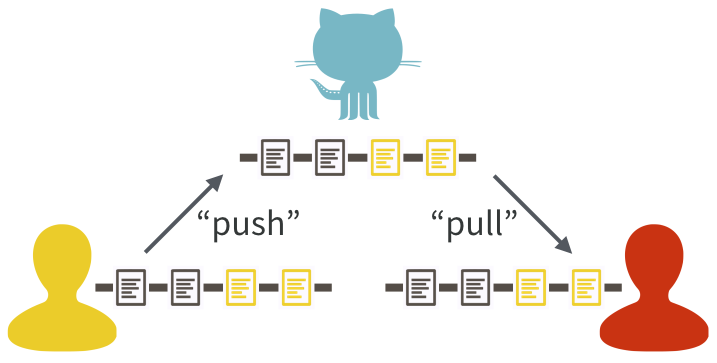
\includegraphics[width=1\linewidth]{push-pull} \caption{\label{fig:push-pull}One contributor has made two new commits and updates the master copy on GitHub with a push. Another contributor stays up-to-date with a pull from GitHub.}\label{fig:push-pull}
\end{figure}

What if two people have made changes to the repository? Imagine that
your collaborator makes a change to a file, commits it locally, and
pushes to GitHub. Meanwhile you also make a different change to the same
file and also commit locally. When you try to push your commit to
GitHub, you will fail because there are commits on GitHub that you do
not have. You must pull from GitHub. The good news is that quite often,
this will ``just work'', i.e.~the GitHub version and your version will
merge cleanly. Git is quite clever at reconciliation and changes to
different files or even distinct parts of the same file will merge. This
derives from the ``diff'' based model of Git described earlier. After a
successful merge, you can push your changes and the cycle goes on.

But sometimes it's not clear how to reconcile your changes with the new
ones from GitHub and you get a \emph{merge conflict}. Merge conflicts
are the most frustrating thing about using Git and GitHub. You can avoid
them if you only work alone, on one computer, but I've also said that
collaboration is the best reason to use GitHub! So this problem must be
confronted.

What is a merge conflict? It happens when Git can't be certain how to
jointly apply the diffs from two different commits to their common
parent. At each location of conflict, you must pick one version or the
other -- or create a hybrid -- and mark it as resolved. Many Git clients
have special tooling for this specific task, which can be very
convenient. Once you've resolved all conflicts, you will be able to
finalize the merge and push a version integrating your recent changes to
GitHub.

The best way to deal with merge conflicts is to prevent them. This is
another reason for all parties to commit, pull, and push often. Small
changes, integrated frequently, in non-binary files, are the easiest for
Git to automatically merge for you. The difficulty of merging (by Git or
by you) is proportional to the evolutionary distance between two lines
of work. The presence of frequently-changing binary files also increases
the burden. So make lots of small commits, sync regularly with GitHub,
and only track binary files with good reason.

\subsection{GitHub as web presence}\label{github-as-web-presence}

Simply having a project on GitHub gives it a web presence! Non-users of
Git/GitHub can visit the project in the browser and interact with it
like a webpage. They can grab a snapshot of all the files as a ZIP
archive by simply clicking a button. People with GitHub accounts can use
Git-specific methods to make their own copy, i.e.~a clone or a fork,
which make it easy to keep current with future changes.

GitHub also offers several ways to host a proper website directly from a
repository, collectively known as
\href{https://help.github.com/categories/github-pages-basics/}{GitHub
Pages}. At one extreme, as long as you've got one Markdown file,
\href{https://github.com/blog/2289-publishing-with-github-pages-now-as-easy-as-1-2-3}{GitHub
Pages can create a simple website} automatically. At the other extreme,
sophisticated users can take full advantage of the
\href{https://jekyllrb.com}{Jekyll static site generator}. The STAT 545
website (\href{http://stat545.com}{stat545.com},
\href{https://github.com/STAT545-UBC/STAT545-UBC.github.io}{GitHub
repo}) falls on the more primitive side.
\href{http://rmarkdown.rstudio.com/rmarkdown_websites.html}{R Markdown
websites}, \href{https://bookdown.org}{bookdown}
\citep{bookdown-pkg, bookdown-book}, and
\href{https://bookdown.org/yihui/blogdown/}{blogdown} provide several
R-focused options for rendering the pages \emph{en masse}.

But even before you make an actual website, certain practices can
\href{http://happygitwithr.com/repo-browsability.html}{make your GitHub
repository much more browsable}. For many projects, this is more than
sufficient for helping people connect with your work.

\textbf{Be savvy about file formats.} Keep files in the plainest,
web-friendliest form that is compatible with your main goals. As
explained above, Markdown is the ideal format for prose, because it is
just plain text with some markup, but will be displayed like HTML on
GitHub. Files named \texttt{README.md} are extra special, acting as the
index or landing page for their host directory.
\href{https://help.github.com/articles/rendering-csv-and-tsv-data/}{CSV
and TSV} files also get special treatment, including an attractive grid
layout and search. GitHub has excellent support for displaying and
diffing common image formats.

\textbf{Use conventional file extensions.} GitHub is very code-aware and
will apply proper syntax highlighting for almost any language you can
think of, if you use one of the standard file extensions. This also has
advantages for people searching GitHub and trying to filter by language.

\textbf{Use internal links.} \texttt{README.md} is a great place to
explain how your project fits together. Any Markdown file can include
relative links to other files in the repo. Embedded images are also
displayed. For figures produced by R code, these links are part of what
rmarkdown takes care of for you, but there's no reason you can't do the
same yourself for any Markdown file.

\subsection{More resources}\label{more-resources}

I've tried to convey the main points about the use of Git and GitHub in
statistical and data analytical settings, but I've had to leave many
things out. There are more advanced topics that will come up once your
use of Git becomes more sophisticated and there are topics that are only
relevant to certain types of reader.

I targeted \href{https://github.com}{GitHub} -- not
\href{https://bitbucket.org}{Bitbucket} or
\href{https://about.gitlab.com}{GitLab} -- for the sake of specificity.
However, all the big-picture principles and even some mechanics will
carry over to these alternative hosting platforms. I am advocating for
the use of hosted version control as a general concept, with GitHub
being the best and most common provider today. I note that many
companies and even universities are starting to make GitHub Enterprise
or GitLab available internally. For example, we host our own instance of
GitHub Enterprise at UBC to support our Master of Data Science program

Don't fret too much about public versus private repositories at this
point. All the major hosting providers offer private repositories with
flexible control over who can read or write to the repo. There are many
ways to get private repositories for low or no cost,
\href{https://help.github.com/articles/discounted-organization-accounts/}{especially
for academics}. If you outgrow this initial arrangement, you can throw
some combination of technical savvy and money at the problem. You can
either pay for a higher level of service, self-host one of these
platforms, or advocate for organization-wide solutions.

Branches and pull requests are an extremely powerful feature of
Git/GitHub and should be your first foray beyond the basics of commit,
push, and pull. A branch is an independent line of development within a
repo, where the intent is usually to merge it into the master branch
when ready. In a course website, you might work in a branch to update a
series of lessons, while leaving the current version intact in the
meantime. A pull request is a GitHub-specific way to propose changes to
a repo that augments Git's regular branch and merge workflow with
facilities for structured review. A pull request can be made between two
branches in the same repo, such as \texttt{master} and \texttt{bugfix},
or between two independent copies of a repo, an original and a so-called
``fork''. This is the mechanism for making and accepting contributions
to open source software projects on GitHub, including many popular R
packages \emph{link to a search?}.

\emph{inspiration for possible figure on collaboration/mergin, from the
barlett talk}

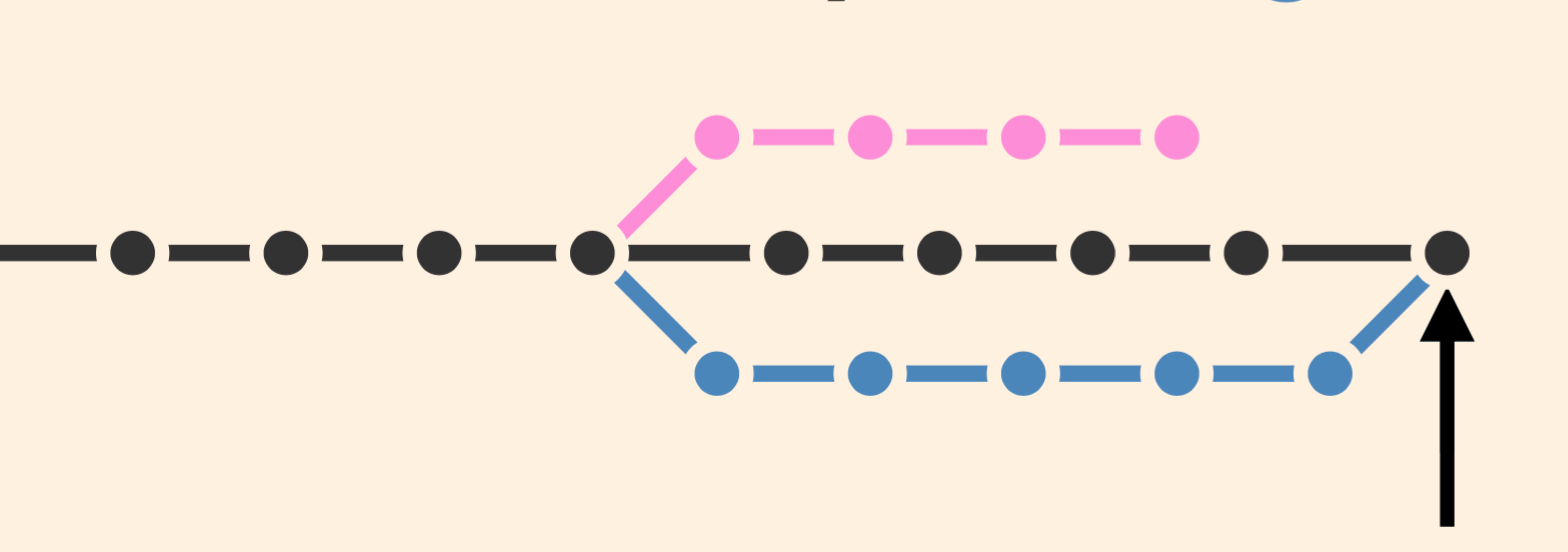
\includegraphics[width=1\linewidth]{img/bartlett-merge-commit}

\subsection{Conclusion}\label{conclusion}

\emph{NEEDS ONE \ldots{} BUT SHORT \ldots{} SOME FODDER}

Transparency about process and product is increasingly important in
science. The SOMETHING for reproducibility is well accepted. A more
underappreciated benefit is democratization of our field, as this
affords a much broader audience a clear view of how scientists and
programmers work.

make statistical thought and implementation available

\bibliographystyle{agsm}
\bibliography{git-github-for-stats.bib}

\end{document}
